Zunächst soll auf die zu analysierenden Oberflächen genauer eingegangen werden.
Die deflektometrischen Verfahren werden explizit für spiegelnde Oberflächen entwickelt.
Doch aus welchem Grund trifft man die Unterscheidung zwischen spiegelnden und nicht-spiegelnden Objekten?
Warum lassen sich Verfahren für diffus reflektierende Oberflächen nicht auch für spiegelnden Oberflächen anwenden?
Zur Beantwortung dieser Fragen sollte man die Eigenschaften der Oberflächen genauer betrachten.
Eine diffus reflektierende Oberfläche strahlt die auftreffenden Lichtstrahlen in viele Richtungen ab, wohingegen spekular reflektierende Oberflächen die Lichtstrahlen in eine Richtung reflektieren.
Diffus reflektierende Oberflächen werden als matt oder rau bezeichnet, weil die Lichtstrahlen auf mikroskopischer Ebene auf eine raue Oberfläche treffen.
Spekular reflektierende Oberflächen werden als spiegelnd oder glatt bezeichnet, weil die Lichtstrahlen auf mikroskopischer Ebene auf eine glatte Oberfläche treffen.
Abbildung \ref{tikz:abbGlattUndRau} zeigt diesen Zusammenhang zwischen der mikroskopischen Oberflächenbeschaffenheit und den daraus folgenden Reflexionseigenschaften.

% Abbildung: Glatte und Raue Oberfläche
{
	\begin{figure}[H]
		\centering
		\begin{adjustbox}{width=\textwidth}
	\begin{tikzpicture}[every node/.style={inner sep=0,outer sep=0}]
	
		\node [anchor=north east] (imgGlatt) at (-0.03\textwidth,0) {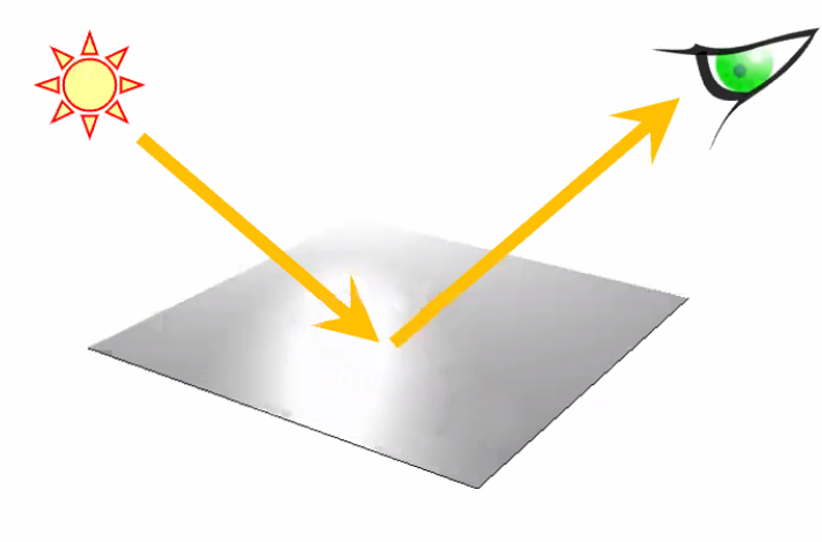
\includegraphics[width=.47\textwidth]{02_grundlagenZurDeflektometrie/spiegelndeOberflaechen/figures/spiegelnd}};
		\node [below=0.2cm of imgGlatt, align=center] {Spiegelnde Oberfläche mit glatter \\ Oberflächenbeschaffenheit};
		\node [anchor=north west] (imgRau) at (0.03\textwidth,0) {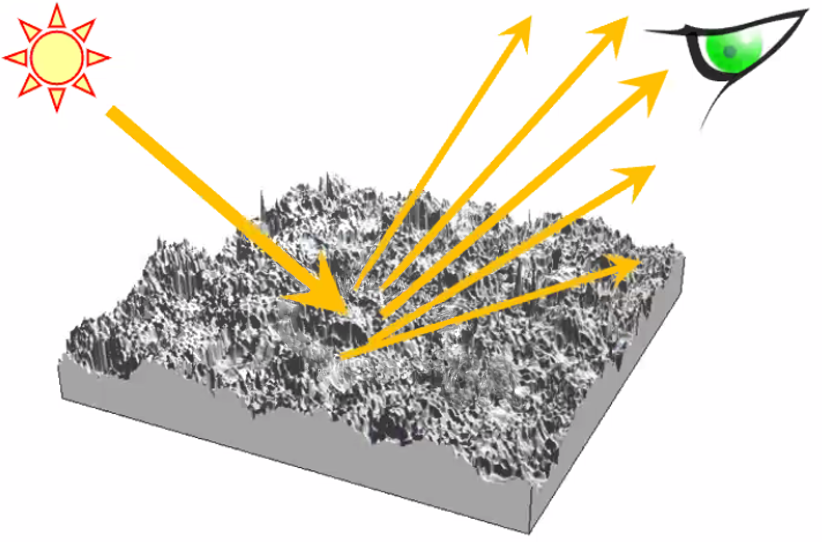
\includegraphics[width=.47\textwidth]{02_grundlagenZurDeflektometrie/spiegelndeOberflaechen/figures/rau}};
		\node [below=0.2cm of imgRau, align=center] {Matte Oberfläche mit rauer \\ Oberflächenbeschaffenheit};
		
	\end{tikzpicture}
\end{adjustbox}
\caption[Spiegelnde und matte Oberflächen]{Spiegelnde bzw. glatte und matte bzw. raue Oberflächen in ihrer mikroskopischer Oberflächenbeschaffenheit. \cite{jenaerOK}}
		\label{tikz:abbGlattUndRau}
	\end{figure}
}
%
\noindent
Durch diese unterschiedliche Reflexionsarten eignen sich für die Oberflächen unterschiedliche Szenen zur Auswertung der Krümmung.
Während spiegelnde Oberfläche ein abbildendes System der Szene darstellt, lässt sich eine Szene über die matte Oberfläche nicht durch eine Spiegelung beobachten.
Für matte Oberflächen eignet sich daher eine Projektion mit viel Licht zur Beobachtung einer Szene.
Für spiegelnde Oberflächen ist dies aufgrund der hohen Reflektivität ungeeignet, stattdessen verwendet man zur Darstellung einer Szene direkt einen Bildschirm (siehe Abbildung  \ref{tikz:abbDeflektometrieVSProjektion}).

% Abbildung: Glatte und Raue Oberfläche
{
	\begin{figure}[H]
		\centering
		\begin{adjustbox}{width=\textwidth}
	\begin{tikzpicture}[every node/.style={inner sep=0,outer sep=0}]
	
		\node [anchor=north east] (imgDeflektometrie) at (-0.03\textwidth,0) {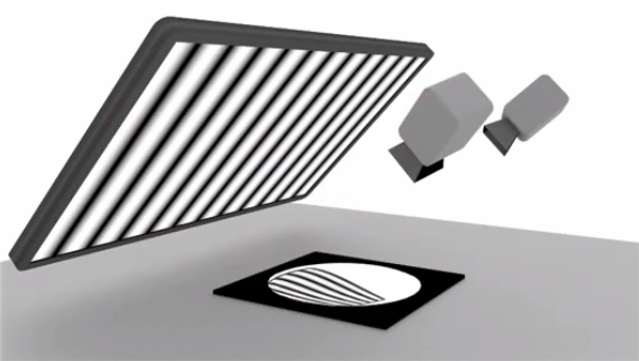
\includegraphics[width=.47\textwidth]{02_grundlagenZurDeflektometrie/spiegelndeOberflaechen/figures/deflektometrie}};
		\node [below=0.2cm of imgDeflektometrie, align=center] {Deflektometrische Verfahren für \\ spiegelnde Oberflächen};
		\node [anchor=north west] (imgProjektion) at (0.03\textwidth,0) {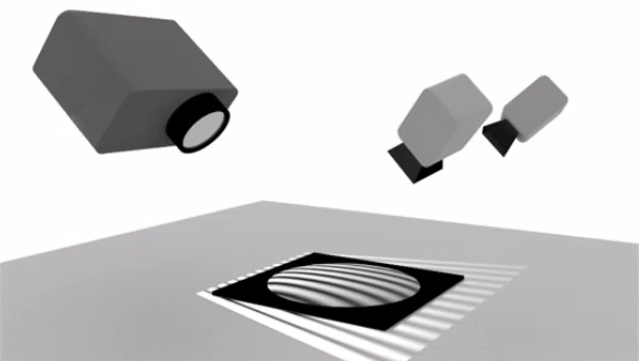
\includegraphics[width=.47\textwidth]{02_grundlagenZurDeflektometrie/spiegelndeOberflaechen/figures/streifenlichtprojektion}};
		\node [below=0.2cm of imgProjektion, align=center] {Streifenlichtprojektion für \\ matte Oberflächen};
		
	\end{tikzpicture}
\end{adjustbox}
\caption[Spiegelnde und matte Oberflächen]{Spiegelnde bzw. glatte und matte bzw. raue Oberflächen in ihrer mikroskopischen Oberflächenbeschaffenheit. \cite{jenaerOK}}
		\label{tikz:abbDeflektometrieVSProjektion}
	\end{figure}
}

\noindent
Im Vergleich erreichen beide Beleuchtungen die Aufnahme einer Szene über der Oberfläche.
Dies ist notwendig um bestimmte Aussagen über die Prüfobjekte treffen zu können.
Der wesentliche Unterschied der beiden Verfahren besteht in der Messempfindlichkeit.
Die deflektometrischen Messverfahren sind neigungssensitiv, da die Reflexion direkt von der Oberflächennormale an den auftreffenden Stellen abhängt.
Im Gegensatz dazu ist die Streifenlichtprojektion durch das Hinzufügen einer Projektionslinse ein höhensensitives Messverfahren für diffus reflektierende Objekte.
Die Oberflächenneigung selbst beeinflusst die aufgenommene Szene bei der Streifenlichtprojektion nicht sehr stark.

\p
Durch die unterschiedliche Funktionsweise der Beleuchtungen für spiegelnde und matte Oberflächen verwendet auch unterschiedliche Verfahren zur Auswertung der Messungen.
Dennoch lassen sich für beide Fälle Analogien in der Auswertung finden, da ein ähnliches Problem betrachtet wird.
Mit diesem Wissen über den Einsatz von bestimmten Beleuchtungen für die jeweiligen Oberflächen, kann man Verfahren beschreiben zur Analyse von spiegelnden Oberflächen.